\documentclass[notitlepage, a4paper, 11pt]{article}

\usepackage{geometry}
\geometry{
	a4paper,
	total={170mm,257mm},
	left=20mm,
	top=20mm,
}

\usepackage{gensymb}
\usepackage{wrapfig}
\usepackage{xcolor}
\usepackage{graphicx}
\usepackage{amsmath}
\usepackage{amssymb}
\usepackage{mathtools}
\usepackage{amsfonts}
\usepackage{listings}
\usepackage{xcolor}
\usepackage{minted}
\usepackage{tikz}
\usepackage[european resistors]{circuitikz}
\usepackage{caption}
\usepackage{subcaption}
\usepackage{hyperref}
\hypersetup{
	pdfborder = false,
	colorlinks=true,
	linkcolor=black,
	filecolor=black,      
	urlcolor=blue,
	pdftitle={Overleaf Example},
	pdfpagemode=FullScreen,
}
\title{Laplace Transform\\
	\large Laboratory III}
\author{Patrycja Nazim, Adrian Król, Gabriel Ćwiek, Kamil Chaj}
\date{}

\begin{document}
	\maketitle
	\section{Goal of the exercise}
	\section{Laplace Transform}
	Laplace transform is an integral transform that converts a function of a real variable(time domain) into a function of complex variable(frequency domain). It is powerful tool for solving differential equations, which turns ODEs into algebraic equations and convolution into multiplication. For function $x(t)$, the Laplace transform is the integral
	
	\begin{equation}
		\mathcal{L}[x(t)] = X(s) = \int_{0}^{\infty}x(t)e^{-st}dt
	\end{equation}
	
	Where $s = \sigma+j\omega$ $\quad \sigma,\omega\in \mathbb{R}$
	\\
	In order to get solution of differential equation solved in s-domain it is necessary to apply inverse Laplace transform which is given by following complex integral
	
	\begin{equation}
		f(t) = \mathcal{L}^{-1}[X(s)] = \dfrac{1}{2\pi j}\int_{c-j\infty}^{c+j\infty}F(s)e^{-st}ds
	\end{equation}
	
	Integrals like these can be quite difficult to solve, that is why lookup table of \href{https://en.wikipedia.org/wiki/Laplace_transform#Table_of_selected_Laplace_transforms}{Laplace transforms} and \href{https://en.wikipedia.org/wiki/Laplace_transform#Properties_and_theorems}{properties} can be very handy.
	\\ \\
	Moving to solving circuits using Laplace transform, there are two approaches, first is constructing differential equation in time domain describing circuit and then solve it using Laplace transform, or second option very similar to solving circuits in steady-state where all components are transformed to s-domain and at the end of calculation transform back to t-domain.
	
	\begin{equation}\label{eq:laplace-rules}
		R \xrightarrow{\mathcal{L}} R \quad C \xrightarrow{\mathcal{L}} \frac{1}{sC} \quad L \xrightarrow{\mathcal{L}} sL
	\end{equation}
	
	
	\section{Course of measurements}
		
		First we tested two circuits: low-pass and high-pass configuration of RC circuit and RLC circuts. After connecting osciloscope to the wave generator and prototype board, we generated square wave with $v_{pp}$ = 1V, $v_{offset}$ = .5V, frequency of 100Hz and duty cycle of 50\%. Then we read from the oscilloscope Voltage value at times 1$\tau$, 5$\tau$ and 10$\tau$ (where 10$\tau$ is just as fail-safe) and time when voltage reaches 10\% and 90\% of the highest value.
		
			\begin{figure}[H]
			\centering
			\begin{subfigure}{0.95\textwidth}
				\centering
				\begin{circuitikz}
					\ctikzset{bipoles/oscope/width=1.5}
					\ctikzset{bipoles/oscope/height=1}
					\draw [black, thick] (0, 0) rectangle (3, -2);
					\node [black, below] at (1.5, -2) {RC circuits};
					\draw [black, thick] (-3, 0) rectangle (-1, -1.5);
					\node [black, above] at (-2, 0) {\small Function Generator};
					\draw (1.5, 1.3) node[oscopeshape](O) {Oscilloscope};
					\node [bnc] at (-1.3, -0.75) (FG) {};
					\node [bnc, font=\tiny, xscale=-1, anchor=zero] at (1, -0.75) (CON1) {};
					\node [bnc, font=\tiny, rotate=90, anchor=zero, label position=45] at (2, -0.75) (CON2) {};
					\node [below, font=\tiny] at (1, -0.85) {CON2};
					\node [below, font=\tiny] at (2, -0.85) {CON1};
					\draw (O.in 1) node[bnc, anchor=zero, rotate=-90](IN1) {};
					\draw (O.in 2) node[bnc, anchor=zero, rotate=-90](IN2) {};
					\draw (FG.hot) to[short, -*] (-0.4, -0.75) -- (-0.4, 0.4) -- (1.08, 0.4) to (IN1.hot);
					\draw (CON1.hot) to[short] (-0.4, -0.75);
					\draw (CON2.hot) to[short] (2, 0.4) -- (1.92, 0.4) -- (IN2.hot);
				\end{circuitikz}
				\caption{Measurement setup}
			\end{subfigure}
			\begin{subfigure}{0.45\textwidth}
				\centering
				\begin{circuitikz}[scale = 0.7, transform shape]
					\draw (0,0) node[bnc](B1) {CON11}
					to[R, l=$R_{11}$, a=1.5k$\Omega$] (3,0)
					to[C, l2=$C_{11}$ and 47nF, l2 halign=c, l2 valign=c] (3,-2)
					node[ground] {}
					;
					\draw (3,0) 
					to[short] (4.5,0)
					node[bnc, xscale=-1](B2){\scalebox{-1}[1]{CON12}}
					;
					\draw node[ground] at (B1.shield) {};
					\draw node[ground] at (B2.shield) {};
				\end{circuitikz}
				\caption{Circuit A}
				\label{fig:Circuit A}
			\end{subfigure}
			\begin{subfigure}{0.45\textwidth}
				\centering
				\begin{circuitikz}[scale = 0.7, transform shape]
					\draw (0,0) node[bnc](B1) {CON21}
					to[C, l=$C_{21}$, a=10nF] (3,0)
					to[R, l2=$R_{21}$ and 1.5k$\Omega$, l2 halign=c, l2 valign=c] (3,-2)
					node[ground] {}
					;
					\draw (3,0) 
					to[short] (4.5,0)
					node[bnc, xscale=-1](B2){\scalebox{-1}[1]{CON21}}
					;
					\draw node[ground] at (B1.shield) {};
					\draw node[ground] at (B2.shield) {};
				\end{circuitikz}
				\caption{Circuit B}
				\label{fig:Circuit B}
			\end{subfigure}
			\caption{RC Circuits}
			\label{fig: Circuit}
		\end{figure}		
		
		For RLC circuits we tested two different resistances before RC circuit influence output characteristic. We measured response for 2 cases: Generator out resistance (50 $\Omega$) + resistance selected by jumper wire. In our case we tested jumper on 1.1k$\Omega$ resistance path and 3.3k$\Omega$. After that we checked response of the circuit:
		\begin{itemize}
			\item if response was sinusoid with decreasing amplitude - resustance was smaller then RC
			\item if response was exp. decay if R was higher
			\item if response was aperiodic critical waveform if resistance was equal RC
		\end{itemize}
		
	
	\begin{figure}[H]
		\centering
		\begin{subfigure}{0.45\textwidth}
			\centering
			\begin{circuitikz}[scale = 0.7, transform shape]
				\node [bnc] at (0,0) (CON41) {};
				\draw (CON41.hot) to[short, -*]
				(1,0) -- (3,0) to[nopb, l_=JP43] (4,0);
				\draw (1,0) -- (1,-2) to[R, l2=$R_{42}$ and $1.1k\Omega$, l2 halign=c, l2 valign=b] (3,-2)
				to[nopb, l_=JP42] (4,-2) -- (4, 0);
				\draw (1,-2) -- (1,-4) to[R, l2=$R_{41}$ and $3.3k\Omega$, l2 halign=c, l2 valign=b] (3,-4)
				to[nopb, l_=JP41] (4,-4) -- (4, -2);
				\draw (4,0) to[short, -*] (5,0)
				to[C, l2=$C_{41}$ and 33nF, l2 halign=c, l2 valign=c] (5,-2) 
				to[L, l2=$L_{41}$ and 10mH, l2 halign=c, l2 valign=c] (5,-4) node[ground] {};
				\draw (5, 0) to (6, 0) node[bnc, xscale=-1, anchor=zero](CON42){};
			\end{circuitikz}
			\caption{Measured Circuit}
		\end{subfigure}
		\hfill
		\begin{subfigure}{0.45\textwidth}
			\centering
			\begin{circuitikz}[scale = 0.8, transform shape]
				\ctikzset{bipoles/oscope/width=1.5}
				\ctikzset{bipoles/oscope/height=1}
				\draw [black, thick] (0, 0) rectangle (3, -3);
				\node [black, below] at (1.5, -3) {RC circuits};
				\draw [black, thick] (-3, 0) rectangle (-1, -1.5);
				\node [black, above] at (-2, 0) {\small Function Generator};
				\draw (4.5, 0.6) node[oscopeshape](O) {Oscilloscope};
				\node [bnc] at (-1.3, -0.75) (FG) {};
				\node [bnc, font=\tiny, xscale=-1, anchor=zero] at (0.5, -0.5) (CON1) {\ctikzflipx{CON1}};
				\node [bnc, font=\tiny] at (2.65, -0.5) (CON2) {CON2};
				\draw (CON2.left) to[short, -*] (1.5, -0.5);
				\draw (CON1.left) to[short, -*] (1.5, -0.5)
				to[C, bipoles/length=7mm] (1.5, -1.25)
				to[L, bipoles/length=10mm] (1.5, -2.5) node[tlground, scale=0.8]{};
				\draw (O.in 1) node[bnc, anchor=zero, rotate=-90](IN1) {};
				\draw (O.in 2) node[bnc, anchor=zero, rotate=-90](IN2) {};
				\draw (FG.hot) -- (-0.5, -0.75) -- (-0.5, -0.5) -- (CON1.hot);
				\draw (CON2.hot) -- (4.08, -0.5) -- (IN1.hot);
				\draw [black, ->](IN2.hot) -- (4.92, -1.35) -- (1.5, -1.35);
				\node [below] at (4.52, -1.3){probe};
			\end{circuitikz}
			\caption{Measurements setup}
		\end{subfigure}
		\caption{RLC circuit}
	\end{figure}

	\newpage
	\section{Theoretical calculations}
	For all calculations we used Matlab with Symbolic Math Toolbox. Source code can be found in Appendix. \ref{sec:appendix}
	\\ \\
	In all three circuit input voltage was square wave with 50\% duty cycle which can be described in time domain by
	
	\begin{equation}
		v_{in}(t) = V_{offset} \mathbf{1}(t) + V_{pp} \mathbf{1}(t-\frac{T}{2}) - V_{pp} \mathbf{1}(t-T)
	\end{equation}
	
	and in frequency domain by
	
	\begin{equation}
		V_{in}(s) = \mathcal{L}[v_{in}(t)] = \frac{V_{offset}}{s} + \dfrac{e^{-\frac{T}{2}s}}{s} - \dfrac{e^{-Ts}}{s}
	\end{equation}

	\subsection{Circuit A}

	First we need to transform circuit to s-domain according to \eqref{eq:laplace-rules}

	\begin{figure}[H]
		\centering
		\begin{circuitikz}[scale = 0.7, transform shape]
			\draw (0,0)
			to[R, l=$R_{11}$, *-] (3,0)
			to[C, l=$\dfrac{1}{sC_{11}}$] (3,-2)
			to[short, -*] (0, -2)
			;
			\draw (0, 0) to[open, v_<=$v_{in}$] (0, -2);
			\draw (3, 0)
			to[short, -*] (5, 0)
			to[open, v^<=$v_{out}$] (5, -2)
			to[short, *-] (3, -2);
		\end{circuitikz}
		\caption{Circuit A schematics}
	\end{figure}
	
	output voltag of circuit A can be described using simple voltage divider
	
	\begin{equation}
		V_{out}(s) = V_{in}(s) \dfrac{\frac{1}{sC_{11}}}{R_{11} +\frac{1}{sC_{11}}}
	\end{equation}
	
	after applying inverse Laplace transform to $v_{out}(s)$ we obtain below plot with marked $\tau$, 5$\tau$, 10$\tau$, 10\% and 90\% of output voltage.
	
	\begin{figure}[H]
		\centering
		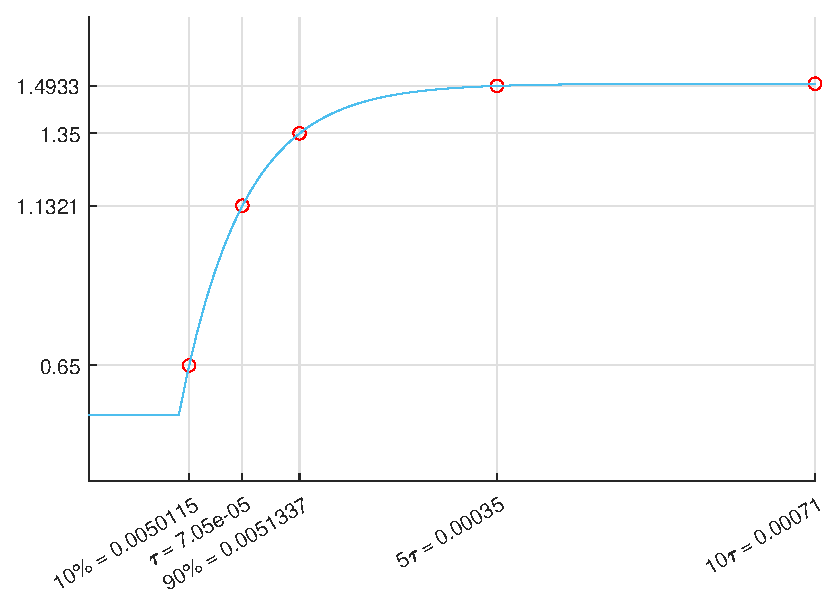
\includegraphics[width=0.5\textwidth]{../Matlab/img/CircuitA.eps}
		\caption{Circuit A output voltage}
	\end{figure}
	
	\newpage
	\subsection{Circuit B}
	steps in circuit B are almost identical to circuit A, first we transformed circuit to s-domain according to \eqref{eq:laplace-rules}
	\begin{figure}[H]
		\centering
		\begin{circuitikz}[scale = 0.7, transform shape]
			\draw (0,0)
			to[C, l_=$\dfrac{1}{sC_{21}}$, *-] (3,0)
			to[R, l=$R_{21}$] (3,-2)
			to[short, -*] (0, -2)
			;
			\draw (0, 0) to[open, v_<=$v_{in}$] (0, -2);
			\draw (3, 0)
			to[short, -*] (5, 0)
			to[open, v^<=$v_{out}$] (5, -2)
			to[short, *-] (3, -2);
		\end{circuitikz}
		\caption{Circuit B schematics}
	\end{figure}
	
	output voltage can be described by voltage divider
	
	\begin{equation}
		V_{out}(s) = V_{in}(s) \dfrac{R_{21}}{R_{21} + \frac{1}{sC_{21}}}
	\end{equation}
	
		after applying inverse Laplace transform to $V_{out}(s)$ we obtain below plot with marked $\tau$, 5$\tau$, 10$\tau$, 10\% and 90\% of output voltage.
	
	\begin{figure}[H]
	\centering
	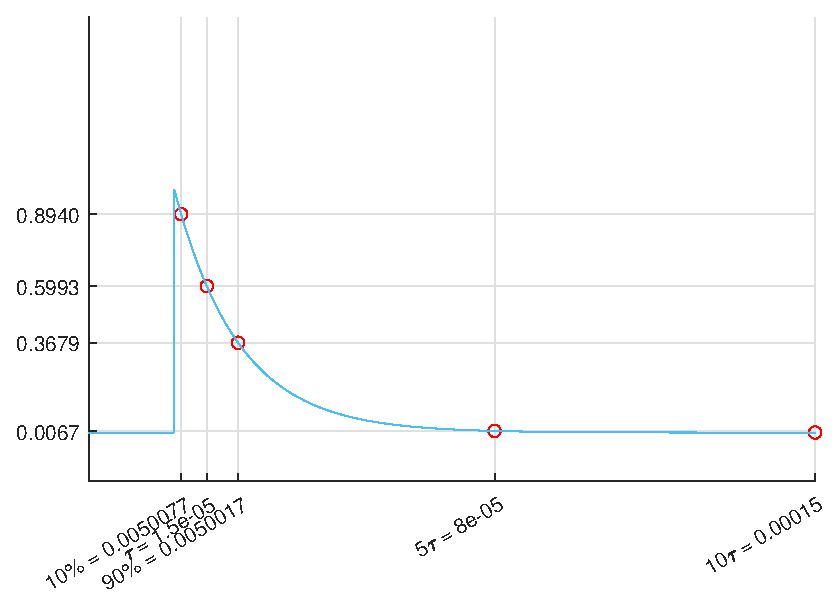
\includegraphics[width=0.5\textwidth]{../Matlab/img/CircuitB.eps}
	\caption{Circuit B output voltage}
\end{figure}
	
	\subsection{Circuit C}
	
	\begin{figure}[H]
		\centering
		\begin{subfigure}{0.8\textwidth}
			\begin{circuitikz}[scale = 0.7, transform shape]
				\draw (0, 0)
				to[R, l2=$R_{in}$ and 50$\Omega$, l2 halign=c, l2 valign=b, *-] (2.5, 0)
				to[short, -*] (5, 0)
				to[open, v^=$v_{out}$] (5, -3) -- (2.5, -3)
				to[L, l2_=$L_{41}$ and 10mH, l2 halign=c, l2 valign=c] (2.5, -1.5)
				to[C, l2_=$C_{41}$ and 33nF, l2 halign=c, l2 valign=c] (2.5, 0);
				\draw (0, 0)
				to[open, v=$v_{in}$](0, -3)
				to[short, -*] (2.5, -3);
			\end{circuitikz}
		\end{subfigure}
		
		\begin{subfigure}{0.8\textwidth}
			\begin{circuitikz}[scale = 0.7, transform shape]
				\draw (0, 0)
				to[R, l2=$R_{42}$ and 1.1k$\Omega$, l2 halign=c, l2 valign=b] (2.5, 0)
				to[short, *-*] (5, 0)
				to[open, v^=$v_{out}$] (5, -3) -- (2.5, -3)
				to[L, l2_=$L_{41}$ and 10mH, l2 halign=c, l2 valign=c] (2.5, -1.5)
				to[C, l2_=$C_{41}$ and 33nF, l2 halign=c, l2 valign=c] (2.5, 0);
				\draw (0, 0)
				to[open, v=$v_{in}$](0, -3)
				to[short, -*] (2.5, -3);
			\end{circuitikz}
		\end{subfigure}
		
		\begin{subfigure}{0.8\textwidth}
			\begin{circuitikz}[scale = 0.7, transform shape]
				\draw (0, 0)
				to[R, l2=$R_{41}$ and 3.3k$\Omega$, l2 halign=c, l2 valign=b] (2.5, 0)
				to[short, *-*] (5, 0)
				to[open, v^=$v_{out}$] (5, -3) -- (2.5, -3)
				to[L, l2_=$L_{41}$ and 10mH, l2 halign=c, l2 valign=c] (2.5, -1.5)
				to[C, l2_=$C_{41}$ and 33nF, l2 halign=c, l2 valign=c] (2.5, 0);
				\draw (0, 0)
				to[open, v=$v_{in}$](0, -3)
				to[short, -*] (2.5, -3);
			\end{circuitikz}
		\end{subfigure}
	\end{figure}
	
	\section{Comparison}
	\section{Conclusions}
	
	\newpage
	\appendix
	\section{Appendix}\label{sec:appendix}
\end{document}